\documentclass[a4paper,11pt]{article}
\usepackage{amssymb}
\usepackage{booktabs}
\usepackage{geometry}
\usepackage{color}
\usepackage{hyperref}
\usepackage{listings}
\usepackage{graphicx}
\usepackage{float}
\usepackage{caption}
\usepackage{subcaption}
\usepackage[T1]{fontenc}
\usepackage{algo}

\geometry{
	includeheadfoot,
	margin=2.54cm
}

\setlength\parindent{24pt}

\title{
	2IL76 Algorithms for Geographic Data Set 3 \\
}
\author{
	Bram Kohl - b.j.e.kohl@student.tue.nl - 0746107
}
\date{\today}

\begin{document}
	\maketitle
	
\section*{Exercise 1}
Average speed $\geq \delta$ is neither monotone decreasing, nor increasing. Take for example figure \ref{fig:trajectory1}, and $\delta = 2$.

\begin{figure}[H]
	\centering
	\includegraphics[scale=0.8]{trajectory1}
	\caption{Trajectory to show that average speed $\geq \delta$ is not monotone increasing, nor monotone decreasing}
	\label{fig:trajectory1}
\end{figure}

This example shows both that the average speed $\geq \delta$ property is not monotone decreasing and that it is not monotone increasing. We first show it is not monotone decreasing and thereafter that it is not monotone increasing. \\

Monotone decreasing means that if the property holds on a segment, then it holds for any subsegment as well. In the given example, the average speed of the segment from $a_2$ until $a_4$ is 2, which is equal to $\delta$ so the property holds for that segment. But the average speed of the segment from $a_3$ to $a_4$ is only 1. So for this subsegment of $a_2$-$a_4$, the property does not hold! Thus, the property average speed $\geq \delta$ is not monotone decreasing.\\

Similarly, the average speed $\geq \delta$ property is not monotone increasing. For it to be so, if a segment has the property, any supersegment should have it as well. In the example, the segment from $a_2$ until $a_4$ (still) has average speed 2, which is equal to $\delta$ so the property holds for that segment. But the average speed of the segment from $a_1$ to $a_4$ is $\frac{5}{3}$, so this is $< \delta$. So for this supersegment of $a_2$-$a_4$, the property does not hold! Thus, the property average speed $\geq \delta$ is not monotone increasing.\\\\

In order to find the maximum duration subtrajectory with average speed at least $\delta$, we can use a variation on the \textsc{Longest\_Segment} algorithm from the following paper by Kuan-Yu Chen, and Kun-Mao Chao: \url{http://www.csie.ntu.edu.tw/~kmchao/papers/2005_IPL_Longest.pdf}. \\
\newpage
\begin{algorithm}{My\_Longest\_Segment}{(A)}
	M[0] \qlet D[0] \qlet 0; x \qlet y \qlet 0;\\
	\qfor i \qlet 1 to n \\
		D[i] \qlet D[i-1] + ($||a_i - a_{i-1}||$) - $\delta$\\
		\qif D[i-1] $<$ D[M[i-1]] \\
			\qthen M[i] \qlet i - 1 \\
			\qelse M[i] = M[i-1] \qend \\	
		$k$ \qlet $i-y+x-1$\\
		\qwhile $k > 0$ \\
			\qif D[i] - D[M[k]] $\geq$ 0\\
			\qthen k \qlet M[k] \\
			\qelse \textit{break} \qend \\
		$x$ \qlet $k+1$; $y$ \qlet $i$ \qend \\
		OUTPUT A(x,y) \qend \\
\end{algorithm} 

So the difference with the algorithm in the paper is that we use D instead of C and calculate it a bit different, so it is the same as the D of the assignment. And furthermore we changed L into 0.\\

This algorithm first calculates the value for D as it is defined in the assignment. Furthermore, it keeps track of another array, M, which holds the index for the smallest value of D so far. Lastly, we check whether $D_i$ - $D_{M[k]}$ (which is the segment from the index that had the smallest value of D so far up to the current index) is at least 0. If it is, then the average speed on this segment is at least $\delta$. If this is the case, we set $k$ to be the index and set x and y to the indexes of the start and end vertices of this segment. This way, we start looking for greater segments ending at $i$.

\subsection*{Proof of correctness}
In order to prove the correctness of this algorithm we have to show that the segment it finds has an average speed of at least $\delta$, and that there is no longer segment which has an average speed of at least $\delta$. I would do this by assuming there is a longer segment which has this property and then deducing a contradiction. Unfortunately I do not have any time left to finish this.

\subsection*{Running time}
The outer loop obviously takes O($n$) time. The inner while loop takes O($n$) at most over all the loops together, as the same $k$ is used in each iteration of the outer loop. So in total we get a running time of O($n$).



\section*{Exercise 2}
We are given the trajectory and the subcurve for which we have to find recurrences. We can do this by creating a free space diagram, with on the horizontal axis the points in the given trajectory (A[i,j]) and on the vertical axis all other points. Then we fill this diagram by checking for each of the $n-l$ points on the vertical axis whether it is close to any of the $l$ points in the given trajectory ($< \varepsilon$), and coloring the cell in the diagram black if not. We add an extra row for A[i,j] with all black cells, to prevent finding a solution that jumps from A[i-1] to A[j+1] (more on how we find this solution later).\\

Take for example the curve in figure \ref{fig:curve1}, with $i = 2$ and $j = 3$. Now we would expect $a_2$ to be close to $a_6$ and $a_3$ to be close to $a_7$. Of course, this depends on $\varepsilon$, but let's assume $\varepsilon$ is of a size where this is the case, and no other points are close to $a_2$ or $a_3$.

\begin{figure}[H]
	\centering
	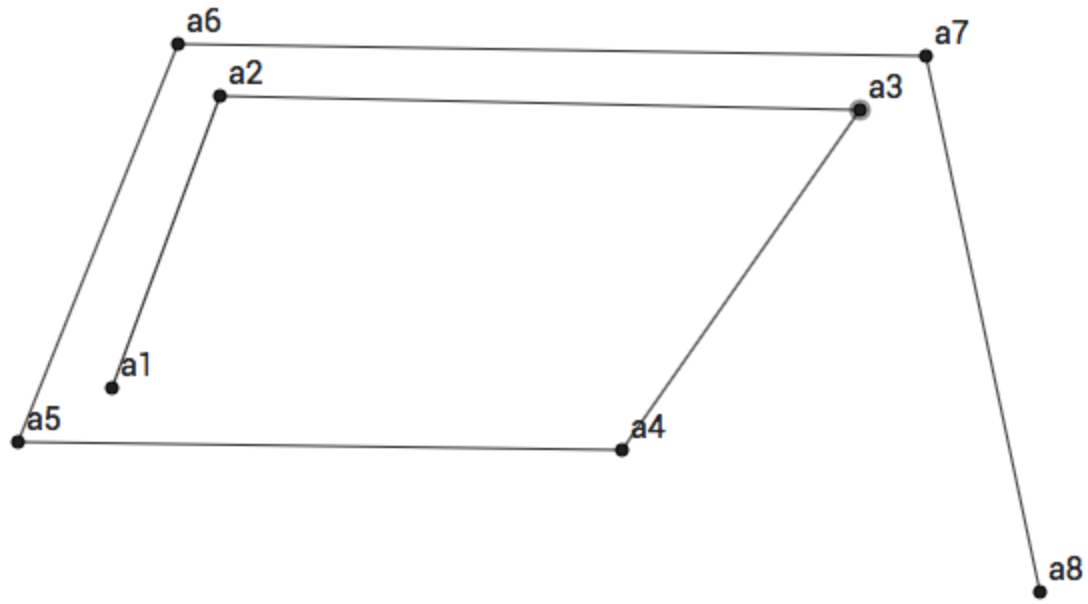
\includegraphics[scale=0.5]{curve1}
	\caption{Curve with recurring subcurve}
	\label{fig:curve1}
\end{figure}

Applying the algorithm that creates the free space diagram then results in the free space diagram of figure \ref{fig:freespace}.

\begin{figure}[H]
	\centering
	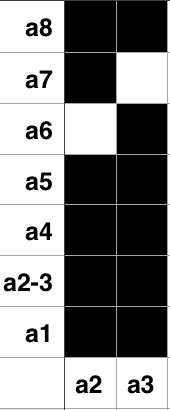
\includegraphics[scale=0.8]{freespace}
	\caption{Free space diagram for figure \ref{fig:curve1}}
	\label{fig:freespace}
\end{figure}

Now, in order to find a solution, we find the lowest free cell in the A[i] column, which in the example is cell ($a_6$,$a_2$). Then we try finding a subcurve by traversing the diagram, prioritizing going to the cell on the right over going to the cell on the top right, and going to the cell one the top right over going to the cell above. We do this to maximize $m$, as we cannot use an A[i] in multiple subcurves, so if we go up, that cell can no longer be used in another subcurve. When we find a subcurve (that is, we get to the $a_j$ column), we start looking for another subcurve with a small enough Fr\'{e}chet distance. We do this by again finding the lowest free cell in the A[i] column, but this time we only look above the cells we used. So in the example we would start looking at $a_7$, which is not free, so we look at $a_8$ which is not free either, so we conclude there are no more subcurves which are close enough to A[i,j]. When we do find such a free cell, we repeat the same process of going right, up right or up.

\subsection*{Proof of correctness}
In order to prove the correctness of our solution, we need to show that the subcurves we find meet the requirements of having a small enough Fr\'{e}chet distance to A[i,j] and being disjoint, as well as show that there is no greater set of subcurves which meet these requirements.\\

For the first part, let's first show that the Fr\'{e}chet distance is small enough. When we find a subcurve A[$i_k$,$j_k$] in the free space diagram, we found it by going to the right, the top right and/or up. So the first vertex of the subcurve, A[$i_k$], is close to A[i]. Then we can separate three cases: we go right, in which case A[$i_k$] is close to A[i+1] as well, we go to the top right, in which case A[$i_k+1$] is close to A[i+1], or we go up, in which case A[$i_k+1$] is close to A[i]. As we stop and add the subcurve only when we reach the A[j] column, and every point in between was close to a point in the other subcurve, the subcurves are close enough to eachother. We do not go back in time in any of the three possible steps (we don't go down or left), so the Fr\'{e}chet distance is small enough.\\
The found subcurves are disjoint, as when we find a subcurve, we continue one row above the last cell in the found subcurve (and this is the highest cell as we never went down). So we can never use one of the used vertices in a new subcurve.\\

What is left to prove is that we find the maximal number of subcurves (maximum $m$) in this way. This is the case, as we go right as much as possible. Only when this is not possible we go upright and when that is not possible either, we go up. So we find the lowest possible subcurve first, and then find the lowest one above that, etc. So using this greedy approach we find the maximum number of subcurves that meet the constraints.

\subsection*{Running time}
Creating the free space diagram just means checking whether the distance between each of the $n-l$ points that are not in the given subcurve A[i,j] and each of the $l$ points in A[i,j] is less than $\varepsilon$. This takes O($nl-l^2$) time. %TODO Traversing the free space diagram takes at most O($n-l + l$) = O($n$) time, as we never go down or left. %<-- NO, failing paths...

\end{document} 